\documentclass[]{article}
\newcommand{\FileDepth}{../../..}
\usepackage[letterpaper, landscape, margin=0.5cm]{geometry}
\usepackage[T1]{fontenc}
\usepackage{textcomp}%Not strictly necessary, but gives \textmu command for "micro."
\usepackage{fancyhdr}
\usepackage{amsmath}
\usepackage{amssymb}
\usepackage{graphicx}
\usepackage{xcolor}
\usepackage{tikz}
\usetikzlibrary{calc}
\usepackage[shortlabels]{enumitem}
\usepackage{multicol}
\usepackage{vwcol}
\usepackage{hyperref}
\usepackage{wrapfig}
%opening
\newcommand{\SecType}{L}
\newcommand{\Week}{6}
\title{PH 211 Lecture \Week}
\author{Benjamin Bauml}
\date{Summer 2024}

\newcommand{\Purpose}{4}
\newcommand{\DefOnly}{0}

% Version 2024-06-14
% Changes
% 2024-02-21 Added xstring package to enable smooth implementation of new \ModePage command.
% 2024-04-27 Set up to split activities and formatting aspects into separate files. Removed dependence on xcomment. Added an automatic counter to number the activities in a problem set.
% 2024-05-19 Revised old format for \TeachingTips command, which did not support \DefOnly.
% 2024-06-14 Added Repurpose environment to allow mixing of different purpose levels in the same document.
\usepackage{tcolorbox}
\usepackage{xstring}
% You will want the following four lines in your document (the last two uncommented):
% For Assignment, leave Purpose as 1. For Worksheet, set to 2. For Student Solution, set to 3. For Teacher Solution, set to 4.
% If you want keep the pieces from being called manually, set DefOnly to 0.
%\newcommand{\Purpose}{4}
%\newcommand{\DefOnly}{1}
\newcommand{\Exclusion}{0}
\newcommand{\PageTurn}{0}
\newcommand{\GrayProb}{0}
\newcommand{\Tipsy}{0}

% Assignment
\if\Purpose1
\renewcommand{\Exclusion}{1}
\fi
% Worksheet
\if\Purpose2
\renewcommand{\Exclusion}{1}
\renewcommand{\PageTurn}{1}
\fi
% Student Solution
\if\Purpose3
\renewcommand{\PageTurn}{1}
\renewcommand{\GrayProb}{1}
\fi
% Teaching Copy
\if\Purpose4
\renewcommand{\PageTurn}{1}
\renewcommand{\GrayProb}{1}
\renewcommand{\Tipsy}{1}
\fi

\newenvironment{Repurpose}[1]{
\renewcommand{\Purpose}{#1}
\renewcommand{\Exclusion}{0}
\renewcommand{\PageTurn}{0}
\renewcommand{\GrayProb}{0}
\renewcommand{\Tipsy}{0}
% Assignment
\if\Purpose1
\renewcommand{\Exclusion}{1}
\fi
% Worksheet
\if\Purpose2
\renewcommand{\Exclusion}{1}
\renewcommand{\PageTurn}{1}
\fi
% Student Solution
\if\Purpose3
\renewcommand{\PageTurn}{1}
\renewcommand{\GrayProb}{1}
\fi
% Teaching Copy
\if\Purpose4
\renewcommand{\PageTurn}{1}
\renewcommand{\GrayProb}{1}
\renewcommand{\Tipsy}{1}
\fi
}{}

\def \NewQ {0}
\def \PForce {0}
\newcommand{\MaybePage}[1]{
	\def \PForce {#1}
	\if\PForce1
	\newpage
	\else
	\if\NewQ0
	\gdef \NewQ {\PageTurn}
	\else
	\newpage
	\fi
	\fi
}

\newcommand{\ModePage}[1]{
	\IfSubStr{#1}{\Purpose}{\newpage}{}
}

\newcounter{ActNumber}
\setcounter{ActNumber}{0}

\newcommand{\Problem}[4][0]{%The first argument is optional, and if it is set to 1, the \newpage will be forced. The second argument is the name of the activity, the third is the command the activity is stored as, and the fourth is the actual problem statement.
\newcommand{#3}{
\MaybePage{#1}
\addtocounter{ActNumber}{1}
\section*{\SecType\Week-\theActNumber: #2}
\if\GrayProb1
\begin{tcolorbox}[colback=lightgray,colframe=lightgray,sharp corners,boxsep=1pt,left=0pt,right=0pt,top=0pt,bottom=0pt,after skip=2pt]
\else
\begin{tcolorbox}[colback=white,colframe=white,sharp corners,boxsep=1pt,left=0pt,right=0pt,top=0pt,bottom=0pt,after skip=2pt]
\fi
#4
\end{tcolorbox}\noindent
}
\if\DefOnly0
\else
#3
\fi
}
	
\newcommand{\ProblemSub}[3][0]{%The first argument is optional, and if a string of numbers is entered into it, it will force a \newpage in any \Purpose that shows up in the string. For example, "13" would lead to the newpage being forced in modes 1 and 3. The second is the command the activity is stored as, and the third is the actual problem statement.
\newcommand{#2}{
\ModePage{#1}
\if\GrayProb1
\begin{tcolorbox}[colback=lightgray,colframe=lightgray,sharp corners,boxsep=1pt,left=0pt,right=0pt,top=0pt,bottom=0pt,after skip=2pt]
\else
\begin{tcolorbox}[colback=white,colframe=white,sharp corners,boxsep=1pt,left=0pt,right=0pt,top=0pt,bottom=0pt,after skip=2pt]
\fi
#3
\end{tcolorbox}\noindent
}
\if\DefOnly0
\else
#2
\fi
}
		
\newcommand{\Solution}[2]{%The first argument is the command the solution is stored as, and the second is the actual solution.
\newcommand{#1}{
\if\Exclusion0
#2
\fi
}
\if\DefOnly0
\else
#1
\fi
}
		
\newcommand{\ProblemFig}[2]{%The first argument is the command the figure is stored as, and the second is the actual figure.
\newcommand{#1}{
\begin{figure}[h]
#2
\end{figure}
}
\if\DefOnly0
\else
#1
\fi
}

\newcommand{\TeachingTips}[2]{%The first argument is the command the tip is stored as, and the second is the actual tip.
\newcommand{#1}{
\if\Tipsy1
\begin{tcolorbox}[colback=lightgray,colframe=black]
#2
\end{tcolorbox}
\fi
}
\if\DefOnly0
\else
#1
\fi
}
\usepackage[absolute]{textpos}
% This package relies on Assignment Format 2024-06-14 or later to work. It is recommended that the Purpose and DefOnly commands be given as such:
%\newcommand{\Purpose}{4}
%\newcommand{\DefOnly}{0}
% Activities need to be entered outside of the TeacherMargin and PresentSpace environments, otherwise they will be defined only locally. They can even go in the preamble.
\newenvironment{TeacherMargin}{\begin{textblock*}{10.8cm}(0.5cm,0.5cm)
\small}{\end{textblock*}
\hspace{0.1cm}}
\newenvironment{PresentSpace}{\begin{textblock*}{0.3cm}(26.85cm,9.35cm)
--
\end{textblock*}
\begin{textblock*}{0.3cm}(26.85cm,18.7cm)
--
\end{textblock*}
\begin{textblock*}{0.3cm}(26.85cm,12.24cm)
	--
\end{textblock*}
\begin{textblock*}{15.6cm}(11.8cm,0.5cm)
\begin{Repurpose}{1}
\Large}{\end{Repurpose}
\end{textblock*}
\hspace{0.1cm}}

%\newcommand{\FBDaxes}[3]{
	\begin{scope}[shift={(#1)},rotate=#2]
		% x-axis
		\draw[thick,->] (-2,0) -- (2,0);
		\node[anchor=west] at (2,0) {$x$};
		% y-axis
		\draw[thick,->] (0,-2) -- (0,2);
		\node[anchor=west] at (0,2) {$y$};
		\coordinate (#3) at (0,0);
	\end{scope}
}
\newcommand{\FBDvectorMA}[4]{
	\begin{scope}[shift={(#1)}]
		\coordinate (#4tip) at ({#2*cos(#3)},{#2*sin(#3)});
		\draw[ultra thick,blue,->] (#1) -- (#4tip);
	\end{scope}
}
\newcommand{\FBDvectorXY}[3]{
	\begin{scope}[shift={(#1)}]
		\coordinate (#3tip) at (#2);
		\draw[ultra thick,blue,->] (0,0) -- (#3tip);
	\end{scope}
}
\newcommand{\FBDdot}[1]{
	\filldraw[black] (#1) circle (3pt);
}
%\newcommand{\MVec}[3][0]{%Creates a momentum vector of length #3 centered at #2 and rotated #1 degrees counterclockwise.
	\begin{scope}[rotate=#1,shift={(#2)}]
		\draw[->,thick] ({-#3/2},0) -- ({#3/2},0);
	\end{scope}
}
\newcommand{\MDot}[1]{%Creates a dot at #1 to represent a zero vector.
	\filldraw (#1) circle (1pt);
}
\newcommand{\MVDRows}[2][4.5]{%Creates the rows (initial, delta, final) of a momentum vector diagram. The optional argument determines the width of the table, and defaults to a good length for three columns (two objects and the total system). The non-optional argument gives a coordinate name (not displayed) to the diagram.
	\begin{scope}
		%\draw[thick] (0,5.5) -- (0,0);
		\draw[thick] (-1,4.5) -- (#1,4.5);
		\node at (-0.5,3.75) {$\vec{p}_{i}$};
		\draw[thick] (-1,3) -- (#1,3);
		\node at (-0.5,2.25) {$\Delta\vec{p}$};
		\draw[thick] (-1,1.5) -- (#1,1.5);
		\node at (-0.5,0.75) {$\vec{p}_{f}$};
		\coordinate (#2) at (0,5);
	\end{scope}
}
\newcommand{\MVDCol}[4][0.75]{%Creates a column for an object in a momentum vector diagram. The first (non-optional) argument is the coordinate name (not displayed) of the column, while the second is the displayed column header. The first argument also names the three entries down the column. The third argument anchors the column, so it should either be the coordinate name of the MVD (for the first column) or the coordinate name of the previous column. The optional argument indicates how far the center of the column should be from the previous column's edge, and defaults to 0.75
	\begin{scope}[shift={(#4)}]
		\node at (#1,0) {#3};
		%\draw[thick] ({#1*2},0.5) -- ({#1*2},-5);
		\draw[thick] (0,0.5) -- (0,-5);
		\coordinate (#2init) at (#1,-1.25);
		\coordinate (#2delt) at (#1,-2.75);
		\coordinate (#2fin) at (#1,-4.25);
		\coordinate (#2) at ({#1*2},0);
	\end{scope}
}

%\input{\FileDepth/Activities/Activity_One/Activity_One.tex}
%\input{\FileDepth/Activities/Activity_Two/Activity_Two.tex}

\begin{document}
\begin{TeacherMargin}
\begin{center}
\begin{tikzpicture}
	\draw[thick] (0,0) node[anchor=south] {Start} -- (0,-5) -- (3,-5) node[anchor=south east,shift={(-0.25,0)}] {$\theta$} node[anchor=west] {End} -- cycle;
	\node[anchor=south west] at (1.5,-2.5) {$d$};
	\draw[thick,->] (1.5,-5.5) -- (1.5,-7);
	\node[anchor=west] at (1.5,-6.25) {Special Case};
	\draw[thick,shift={(3,-7.5)},rotate=59] (-3,5) node[anchor=south] {Start} -- (-1.5,2.5) node[anchor=south] {$d$} -- (0,0) node[anchor=south] {End};
\end{tikzpicture}
\end{center}
If you are sitting on flat ground, waiting to spontaneously start to slide across the floor, you will be waiting for a very long time. In this special case, the answer is (C); it will take an infinite amount of time to reach the end of a horizontal ramp.
\end{TeacherMargin}
\begin{PresentSpace}
\begin{center}
	\huge Lecture 6: Projectile Motion I
\end{center}
\parbox{10cm}{
%\begin{multicols}{2}
\underline{Warm-Up Activity}
\begin{itemize}
	\item You slide down the ramp shown, starting from rest. Consider the special case where the ramp is made horizontal.
	\vspace{-8pt}
	\item How long would it take you to reach the end of the ramp in this case?
	\vspace{-8pt}
	%\begin{multicols}{2}
	\begin{enumerate}[(A)]
		\item No time at all.
		\item The same amount of time as when tilted.
		\item An infinite amount of time.
		\item Not enough information.
	\end{enumerate}
	%\end{multicols}
\end{itemize}
%\end{multicols}
}
\end{PresentSpace}
\begin{textblock*}{5cm}(22.3cm,2.5cm)
\Large
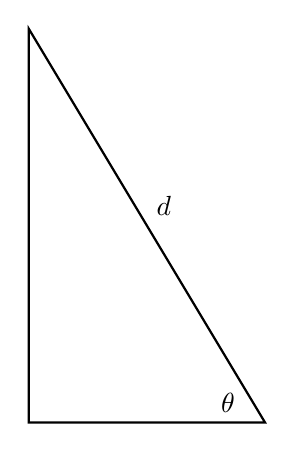
\begin{tikzpicture}
	\draw[thick] (0,0) -- (0,-5) -- (3,-5) node[anchor=south east,shift={(-0.25,0)}] {$\theta$} -- cycle;
	\node[anchor=south west] at (1.5,-2.5) {$d$};
\end{tikzpicture}
\end{textblock*}
\newpage
\begin{TeacherMargin}
\begin{itemize}
	\item $t$ and $\theta$
	\begin{itemize}
		\item It takes an infinite amount of time to slide ``down'' a horizontal ramp.
		\item As $\theta$ decreases toward zero, $\sin\theta$ also decreases toward zero, which means the denominator of the fraction goes to zero. This will cause the fraction (and thus the equation for $t$) to explode to infinity, thus agreeing with our prediction.
	\end{itemize}
	\item $t$ and $d$
	\begin{itemize}
		\item It should take more time to slide down a longer ramp.
		\item According to the equation, increasing $d$ will increase $t$, which matches our prediction.
	\end{itemize}
	\item $t$ and $g$
	\begin{itemize}
		\item If gravity is stronger, then things will be pulled down the ramp faster.
		\item The equation tells us that increasing $g$ will decrease $t$, which matches our prediction.
	\end{itemize}
\end{itemize}
\end{TeacherMargin}
\begin{PresentSpace}
\vspace{-10pt}
\section*{L6-1: Ramp Slide Sensemaking}
\vspace{-10pt}
\parbox{10cm}{
\begin{itemize}
	\item You slide down the ramp shown, starting from rest. Consider the special case where the ramp is made horizontal.
	\item Does the equation below agree with your prediction?
	\[
	t=\sqrt{\frac{2d}{g\sin\theta}}
	\]
	\item Can you make sense of how $t$ depends on $d$ and $g$ as well?
\end{itemize}
}
\end{PresentSpace}
\begin{textblock*}{5cm}(22.3cm,2.5cm)
	\Large
	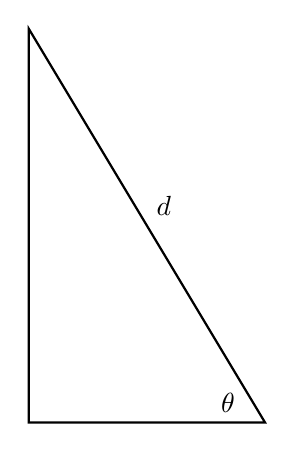
\begin{tikzpicture}
		\draw[thick] (0,0) -- (0,-5) -- (3,-5) node[anchor=south east,shift={(-0.25,0)}] {$\theta$} -- cycle;
		\node[anchor=south west] at (1.5,-2.5) {$d$};
	\end{tikzpicture}
\end{textblock*}
\newpage
\begin{TeacherMargin}
\noindent\textbf{1a) Understand the Problem}
\begin{itemize}
	\item Known:
	\begin{itemize}
		\item $\Delta x = 200$ m, $\theta = 17^{\circ}$
		\item By assumption: $\vec{a}=-g\hat{y}$, $g\approx9.8$ m/s$^{2}$, $\Delta y = 0$ m
	\end{itemize}
	\item Unknown:
	\begin{itemize}
		\item $v_{0}$ (initial speed), $t_{f}$ (time of flight), $v_{f}$ final speed
	\end{itemize}
\end{itemize}
\noindent\textbf{1b) Identify Assumptions}
\begin{itemize}
	\item $\Delta y = 0$ m
	\begin{itemize}
		\item Both the arrow and the target are not going to be at ground level, and archery ranges are typically in flat areas, so for simplicity, it won't be too egregious to assume that the arrow starts and ends at the same height.
	\end{itemize}
	\item The arrow is not affected by moving through air.
	\begin{itemize}
		\item An arrow is fast and aerodynamic, and we don't really know how to handle air resistance or the effects of wind, so we should ignore these effects to make the problem solvable.
	\end{itemize}
	\item Near Earth's surface ($g\approx9.8$ m/s$^{2}$)
	\begin{itemize}
		\item So far, all known archery occurs on Earth, and the height an arrow flies is not significant enough to worry about variation in gravity.
	\end{itemize}
	\item $\vec{a}=-g\hat{y}$
	\begin{itemize}
		\item Since the object is in free-fall with no wind or air effects, and it isn't traveling far enough for the curvature of the Earth to matter, acceleration is straight down and purely gravitational.
	\end{itemize}
\end{itemize}
\noindent\textbf{1c) Represent Physically}
\begin{center}
	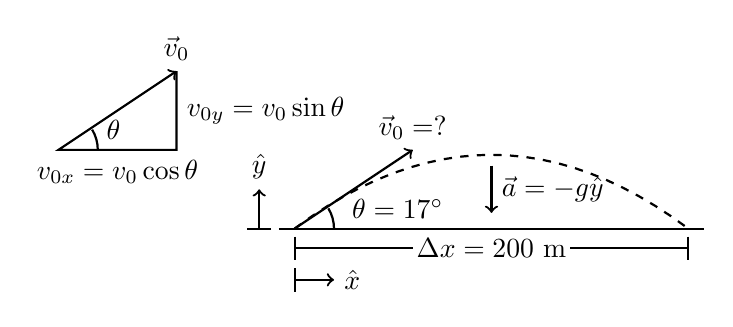
\begin{tikzpicture}
		\begin{scope}[shift={(-3,1)}]
			\draw[thick,->] (1.5,1) node[anchor=west,shift={(0,-0.5)}] {$v_{0y}=v_{0}\sin\theta$} -- (1.5,0) node[anchor=north,shift={(-0.75,0)}] {$v_{0x}=v_{0}\cos\theta$} -- (0,0) node[anchor=south,shift={(0.7,0)}] {$\theta$} -- (1.5,1) node[anchor=south] {$\vec{v}_{0}$};
			\draw[thick] (0.5,0) arc (0:31:0.5);
		\end{scope}
		\begin{scope}
			\draw[thick,->] (0,0) node[anchor=south west,shift={(0.6,0)}] {$\theta=17^{\circ}$} -- (1.5,1) node[anchor=south] {$\vec{v}_{0}=$?};
			\draw[thick,dashed,domain=0:5,variable=\x] plot (\x,{0.75*\x-0.15*\x*\x});
			\draw[thick] (0.5,0) arc (0:31:0.5);
			\draw[thick] (-0.2,0) -- (5.2,0);
			\draw[thick] (0,-0.1) -- (0,-0.4) (5,-0.1) -- (5,-0.4) (0,-0.25) -- (1.5,-0.25) (3.5,-0.25) -- (5,-0.25);
			\node at (2.5,-0.25) {$\Delta x = 200$ m};
			\draw[thick] (0,-0.5) -- (0,-0.8);
			\draw[thick,->] (0,-0.65) -- (0.5,-0.65) node[anchor=west] {$\hat{x}$};
			\draw[thick] (-0.3,0) -- (-0.6,0);
			\draw[thick,->] (-0.45,0) -- (-0.45,0.5) node[anchor=south] {$\hat{y}$};
			\draw[thick,->] (2.5,0.8) -- (2.5,0.5) node[anchor=west] {$\vec{a}=-g\hat{y}$} -- (2.5,0.2);
		\end{scope}
	\end{tikzpicture}
\end{center}
\end{TeacherMargin}
\begin{PresentSpace}
\vspace{-10pt}
\section*{L6-2: Long Distance Archer -- Analyze \& Represent}
\vspace{-10pt}
You are a long-distance archer who releases an arrow that hits a target 200 m away. Your arrow makes an initial angle with the horizontal of $17^{\circ}$. Following the steps for solving an A*R*C*S problem, find the initial speed of the arrow.
\begin{itemize}
	\item \textbf{A}nalyze and \textbf{R}epresent
	\begin{itemize}
		\item Choose appropriate symbols for the quantities you \textbf{know} and \textbf{don't know}.
		\item What assumptions are you making and why are you making them?
		\item Sketch a diagram showing the known and unknown quantities.
	\end{itemize}
\end{itemize}
\end{PresentSpace}
\newpage
\begin{TeacherMargin}
\noindent\textbf{2a) Represent Principles}

\noindent 2-D Kinematics: {\color{blue}Known} {\color{red}Unknown} {\color{purple}Wanted}
\begin{align*}
	{\color{blue}\Delta x} & = v_{0x}{\color{red}t_{f}} + \frac{1}{2}{\color{blue}a_{x}}{\color{red}t_{f}}^{2} & {\color{blue}\Delta y} & = v_{0y}{\color{red}t_{f}} + \frac{1}{2}{\color{blue}a_{y}}{\color{red}t_{f}}^{2} \\
	{\color{red}v_{fx}} & = v_{0x} + {\color{blue}a_{x}}{\color{red}t_{f}} & {\color{red}v_{fy}} & = v_{0y}+{\color{blue}a_{y}}{\color{red}t_{f}} \\
	{\color{red}v_{fx}}^{2} & = v_{0x}^{2} + 2{\color{blue}a_{x}}{\color{blue}\Delta x} & {\color{red}v_{fy}}^{2} & = v_{0y}^{2} + 2{\color{blue}a_{y}}{\color{blue}\Delta y}
\end{align*}
We can avoid the bottom four equations, since we don't really want to know $v_{f}$. \\
Trigonometry:
\begin{align*}
	v_{0x} & = {\color{purple}v_{0}} \cos{\color{blue}\theta} & v_{0y} & = {\color{purple}v_{0}} \sin{\color{blue}\theta}
\end{align*}
\textbf{2b) Find Unknown(s) Symbolically} \\
Between ${\color{blue}\Delta x} = v_{0x}{\color{red}t_{f}} + \frac{1}{2}{\color{blue}a_{x}}{\color{red}t_{f}}^{2}$ and ${\color{blue}\Delta y} = v_{0y}{\color{red}t_{f}} + \frac{1}{2}{\color{blue}a_{y}}{\color{red}t_{f}}^{2}$, we have four knowns ($\Delta x,\ \Delta y,\ a_{x}, a_{y}$) and three unknowns ($t,\ v_{0x},\ v_{0y}$). However, $v_{0x}$ and $v_{0y}$ are components of $\vec{v}_{0}$, and we know $\theta$, so they are sort of a single shared unknown, as is time. Two equations sharing two unknowns can be solved.
\begin{align*}
	{\color{blue}\Delta y} & = v_{0y}{\color{red}t_{f}} + \frac{1}{2}{\color{blue}a_{y}}{\color{red}t_{f}}^{2} & {\color{blue}\Delta x} & = v_{0x}{\color{red}t_{f}} + \frac{1}{2}{\color{blue}a_{x}}{\color{red}t_{f}}^{2} \\
	0 & = v_{0y}t_{f} - \frac{1}{2}gt_{f}^{2} & \Delta x & = v_{0x}\frac{2v_{0y}}{g} + 0 \\
	& = \left(v_{0y} - \frac{1}{2}gt_{f}\right)t_{f} & & = \frac{2v_{0}^{2}}{g}\cos\theta\sin\theta \\
	0 & = v_{0y} - \frac{1}{2}gt_{f} & v_{0} & = \sqrt{\frac{\Delta x g}{2\sin\theta\cos\theta}} \\
	t_{f} & = \frac{2v_{0y}}{g} & & = \sqrt{\frac{\Delta x g}{\sin(2\theta)}}
\end{align*}
\textbf{2c) Plug in Numbers}
\[
v_{0} = \sqrt{\frac{(200\text{ m})(9.8\text{ m/s}^{2})}{\sin(2\times17^{\circ})}} \approx \sqrt{\frac{19600}{0.559}\frac{\text{m}^{2}}{\text{s}^{2}}} \approx 59.2 \text{ m/s}
\]
If you assume $g \approx 10$ m/s$^{2}$, then $v_{0}\approx59.8$ m/s.
\end{TeacherMargin}
\begin{PresentSpace}
\vspace{-10pt}
\section*{L6-2: Long Distance Archer -- Calculate}
\vspace{-10pt}
You are a long-distance archer who releases an arrow that hits a target 200 m away. Your arrow makes an initial angle with the horizontal of $17^{\circ}$. Following the steps for solving an A*R*C*S problem, find the initial speed of the arrow.
\begin{itemize}
	\item \textbf{C}alculate: Find a \textbf{symbolic expression} for the initial speed of the arrow.
	\begin{itemize}
		\item \textit{Hint 1:} \textbf{Use the symbols you defined before} to help you choose which kinematics equatiosn to use for the $x$- and $y$-directions.
		\item \textit{Hint 2:} Think about which quantity is the same for the $x$- and $y$-directions.
		\item Wait until the end to plug in numbers!
	\end{itemize}
\end{itemize}
\end{PresentSpace}
\newpage
\begin{TeacherMargin}
\noindent\textbf{3a) Units} \\
We want $[v_{0}] = \frac{\text{m}}{\text{s}}$, and we know $[\Delta x]=\text{m}$, $[g]=\frac{\text{m}}{\text{s}^{2}}$, and $[\sin(2\theta)]=1$ (unitless), so
\[
[v_{0}] = \sqrt{\frac{[\Delta x][g]}{[\sin(2\theta)]}} = \sqrt{\frac{\text{m}\cdot\text{m}/\text{s}^{2}}{1}} = \sqrt{\frac{\text{m}^{2}}{\text{s}^{2}}}
\]
Note that I got a bit of a free unit check by plugging in numbers with units in 2c. \\
\textbf{3b) Numbers} \\
Converting into miles per hour, we find that $v_{0} \approx 132$ mph. According to a quick internet search, the speed of a recurve bow shot is around 150 mph (around 204 mph for a compound bow), so we are in the right neighborhood. \\
Side Note: In Olympic archery, the target is set 70 m from the archer, so the given $\Delta x = 200$ m is rather large in comparison to modern competition. \\
\textbf{3c) Symbols}
\begin{itemize}
	\item $\Delta x$ increases
	\begin{itemize}
		\item If the range increases, the arrow must cover a greater distance before it hits the ground, so one would expect it to travel faster.
		\item $v_{0}$ increases as $\Delta x$ increases, so our equation matches this prediction.
	\end{itemize}
	\item $g$ increases
	\begin{itemize}
		\item If $g$ increases (say we do archery on Jupiter), then the arrow will be dragged to the ground more quickly, so it must go faster to cover the same distance in less time.
		\item $v_{0}$ increases as $g$ increases, so our equation matches this prediction.
	\end{itemize}
	In both of the above, it is worth noting that increasing $v_{0}$ not only helps the arrow cover horizontal distance faster, but also increases its time of flight by giving it more vertical speed.
	\item $\theta$ increases
	\begin{itemize}
		\item This one isn't as easy. Note the graph of $\sin(2\theta)$:
		\vspace{-10pt}
		\begin{center}
			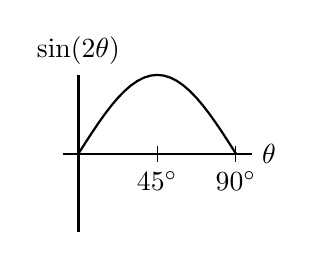
\begin{tikzpicture}
				\draw[thick] (0,-1) -- (0,1) node[anchor=south] {$\sin(2\theta)$};
				\draw[thick] (-0.2,0) -- (2.2,0) node[anchor=west] {$\theta$};
				\draw (1,0.1) -- (1,-0.1) node[anchor=north] {$45^{\circ}$};
				\draw (2,0.1) -- (2,-0.1) node[anchor=north] {$90^{\circ}$};
				\draw[thick,domain=0:2,variable=\x] plot (\x,{sin(90*\x)});
			\end{tikzpicture}
		\end{center}
		\vspace{-10pt}
		\item $\sin(2\theta)$ increases for $0^{\circ}\leq\theta<45^{\circ}$, so $v_{0}$ decreases with increasing $\theta$ for shallower angles.
		\begin{itemize}
			\item At shallow angles, the arrow gains more vertical speed (and thus time of flight) than it loses horizontal speed as $\theta$ increases, so tilting up would increase the range if $v_{0}$ did not decrease.
		\end{itemize}
		\item $\sin(2\theta)$ decreases for $45^{\circ}<\theta\leq90^{\circ}$, so $v_{0}$ increases with increasing $\theta$ for steeper angles.
		\begin{itemize}
			\item At steep angles, the arrow loses more horizontal speed than it gains vertical speed (and thus time of flight) as $\theta$ increases, so tilting up would shorten the range if $v_{0}$ did not increase.
		\end{itemize}
	\end{itemize}
\end{itemize}
\end{TeacherMargin}
\begin{PresentSpace}
\vspace{-10pt}
\section*{L6-2: Long Distance Archer -- Sensemake}
\vspace{-10pt}
You are a long-distance archer who releases an arrow that hits a target 200 m away. Your arrow makes an initial angle with the horizontal of $17^{\circ}$. Following the steps for solving an A*R*C*S problem, find the initial speed of the arrow.
\begin{itemize}
	\item \textbf{S}ensemake
	\begin{itemize}
		\item Check the units of your answer.
		\item Does your number make sense?
		\item Give a physical explanation for how the initial speed of the arrow would change if you increased each variable that your answer depends on.
	\end{itemize}
\end{itemize}
\end{PresentSpace}
\newpage
\begin{TeacherMargin}

\end{TeacherMargin}
\begin{PresentSpace}
\section*{Main Ideas}
\begin{itemize}
	\item We can use the kinematics equations to solve for any quantity of interest when the acceleration is constant.
	\item Motion in 2 dimensions can be broken down into independent motion in each dimension.
\end{itemize}
\end{PresentSpace}
\end{document}